\begin{figure}
  \caption{\label{fig:internee-ages} Counts of interned persons by age and WRA camp}
  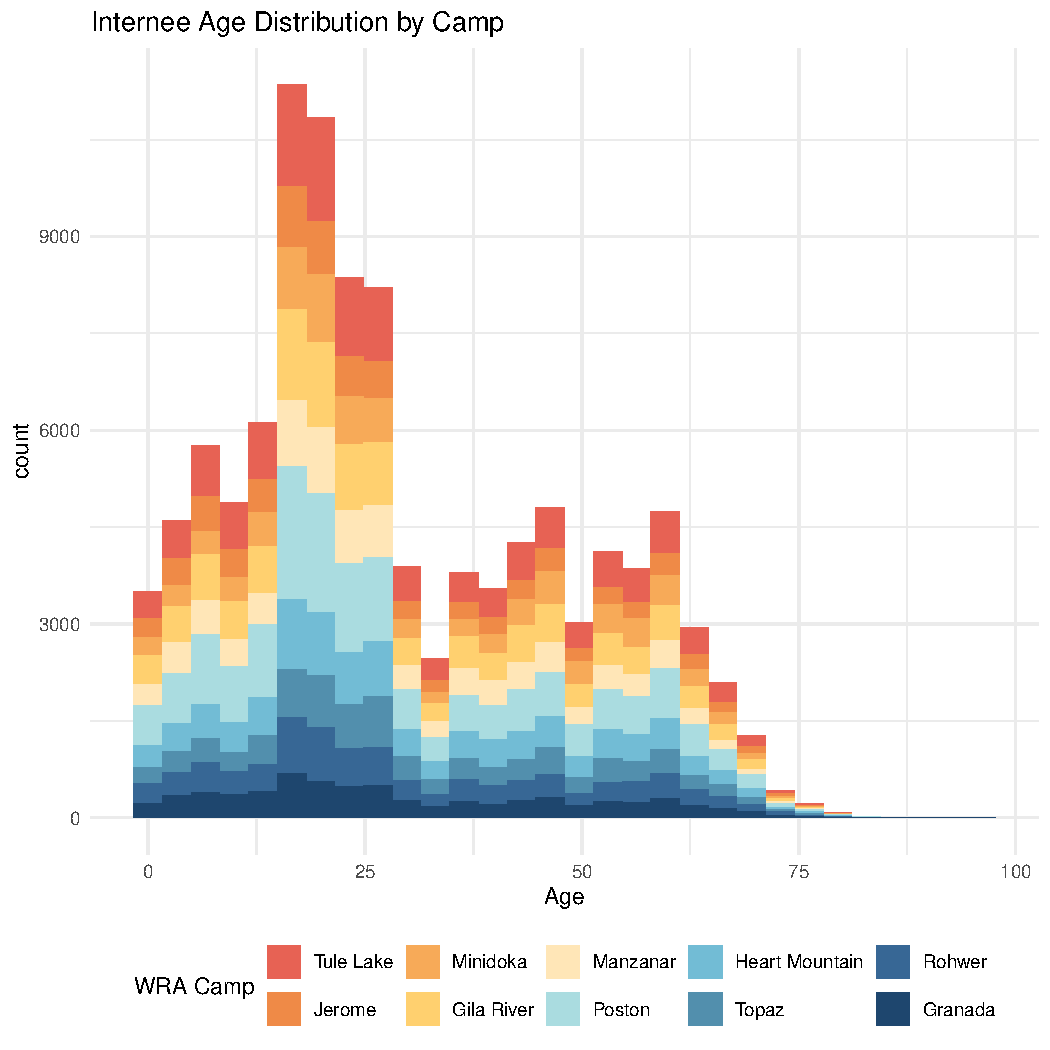
\includegraphics[width=0.6\textwidth]{../figures/internee-age_plot.pdf}
  \footnotesize \\
  Data from the WRA internment camp records on the ages of interned Japanese people in 1942
  infered from their reported birth year. 
  The counts of people in each of the ten internment camps created by the WRA are based on the initial camp they were placed in 
  after being moved from the temporary assembly centers.
\end{figure}
